\documentclass[12pt,a4paper]{article}
\usepackage[T2A]{fontenc}
\usepackage[utf8]{inputenc}
\usepackage[russian]{babel}
\usepackage{geometry}
\geometry{left=2.5cm,right=1.5cm,top=2cm,bottom=2cm}
\usepackage{amsmath,amssymb}
\usepackage{booktabs}
\usepackage{graphicx}
\usepackage{float}
\usepackage{caption}
\usepackage{xcolor}
\usepackage{listings}
\usepackage{hyperref}
\hypersetup{colorlinks=true,linkcolor=blue,urlcolor=blue,citecolor=blue}

\lstset{basicstyle=\ttfamily\small,breaklines=true,frame=single,language=Python,
	commentstyle=\color{gray},keywordstyle=\color{blue}}


\begin{document}
	\tableofcontents
	\newpage
	
	\section{Постановка задачи}
	
	\subsection{Объект и предмет исследования}
	\textbf{Объект исследования:} клеточные автоматы с одним агентом. \textbf{Предмет исследования:} зависимость макроскопического режима поведения агента от строки правил поворота, числа цветов $q$, топологии решётки (квадратная / гексагональная), типа границ и начальных условий поля.
	
	\subsection{Цель и задачи}
	Цель работы --- построить верифицированную классификацию режимов поведения многоцветного муравья Лэнгтона и выявить закономерности их возникновения средствами вычислительного эксперимента. Задачи:
	\begin{enumerate}
		\item формализовать модель в виде $\langle A,S,N,F\rangle$ для квадратной и гексагональной решёток;
		\item реализовать модель и детекторы режимов; провести перекрёстную верификацию независимыми реализациями;
		\item точно измерить параметры магистрали классического муравья (момент возникновения, период, вектор сноса, скорость);
		\item исследовать чувствительность траектории к начальным условиям;
		\item выполнить полный перебор строк правил при $q=2,3,4$ и построить распределения режимов; исследовать мутации одного символа;
		\item сравнить квадратную и гексагональную решётки, открытые, отражающие и периодические границы.
	\end{enumerate}
	
	\subsection{Гипотезы, вынесенные на проверку}
	\begin{itemize}
		\item Классическое правило на пустом поле после длительного хаотического переходного процесса формирует периодическую магистраль; момент перехода не предсказуем аналитически и измеряется только полным моделированием.
		\item С ростом числа цветов $q$ спектр режимов обогащается: появляются неограниченный нерегулярный рост (хаос) и сложные ограниченные режимы.
		\item Точечная мутация строки правил способна изменить класс поведения; пространство правил неоднородно.
		\item Одинаковые правила на разных решётках дают существенно разные результаты: в частности, классическое правило меняет способность строить магистраль при переходе на гексагональную решётку.
		\item В ограниченной коробке конечность фазового пространства гарантирует eventual-периодичность, однако эмпирически длина переходного процесса и цикла превышает доступные времена моделирования; магистраль разрушается первым контактом с границей.
	\end{itemize}
	
	%==================================================================
	\section{Формализация модели}
	%==================================================================
	
	Модель задаётся кортежем $\langle A,S,N,F\rangle$.
	
	\paragraph{Пространство $A$.}
	\begin{itemize}
		\item \emph{Квадратная решётка:} регулярная сетка клеток; агент имеет четыре направления $d\in\{N,E,S,W\}$; в экспериментах с границами поле
		ограничено квадратом $m\times m$ с отражающими или периодическими (тор) границами; в экспериментах без границ поле не ограничено (разреженное представление).
		\item \emph{Гексагональная решётка:} аксиальные координаты $(u,v)$; шесть направлений в порядке по часовой стрелке
		$[(1,0),(0,1),(-1,1),(-1,0),(0,-1),(1,-1)]$; повороты $R,L$ соответствуют $\pm60^\circ$, $U$ --- $180^\circ$.
	\end{itemize}
	
	\paragraph{Состояния $S$.} Клетка: $s\in\{0,1,\dots,q-1\}$, где $q$ --- число цветов ($q=2$ --- классический чёрно-белый случай). Состояние агента: позиция и направление $d$.
	
	\paragraph{Окрестность $N$.} Агент читает только клетку, на которой находится.
	
	\paragraph{Правило $F$.} Задаётся строкой команд длины $q$ над алфавитом
	$\{R,L,F,U\}$. Один такт:
	\begin{enumerate}
		\item считать цвет $s$ текущей клетки;
		\item повернуть согласно команде $rule[s]$;
		\item перекрасить клетку циклически: $s \to (s+1)\bmod q$;
		\item шагнуть вперёд.
	\end{enumerate}
.
	
	\paragraph{Классификация режимов.}
	\begin{enumerate}
		\item \textbf{Класс 1} --- ограниченное движение без обнаруженной периодичности;
		\item \textbf{Класс 2} --- периодическое движение: конфигурация повторяется точно, сдвиг за период $d=(0,0)$;
		\item \textbf{Класс 3} --- магистраль: локальная структура повторяется, агент дрейфует, $d\neq(0,0)$;
		\item \textbf{Класс 4} --- неограниченный нерегулярный рост (хаос);
		\item \textbf{Класс 5} --- симметричный рост.
	\end{enumerate}
	
	\paragraph{Измеряемые показатели.} Расстояние агента от старта (манхэттенское и евклидово); число посещённых клеток; число ненулевых клеток поля; момент возникновения режима $t_{\mathrm{onset}}$; период $\tau$; вектор сноса за период $d$; скорость $v=|d|_1/\tau$; момент первого контакта с границей $t_{\mathrm{wall}}$ и число отражений.
	

	\section{Начальные данные}

	
	\begin{itemize}
		\item Начальное поле во всех базовых прогонах: пустое (все клетки $s=0$).
		\item Начальная позиция агента: центр поля (в ограниченных прогонах) или начало координат (в разреженных); начальное направление $d=N$ ($d=0$).
		\item Длительности: $T=3\cdot10^4$ (перебор правил), $T=1.2\cdot10^4$--$2\cdot10^5$ (целевые прогоны), $T=2\cdot10^5$ (эксперименты с границами).
		\item Размеры коробок: $m\in\{30,50,70\}$; поле без границ: разреженный словарь (неограниченное) либо матрица $1500\times1500$ (визуализация).
	\end{itemize}
	
	Начальные конфигурации Серии~2 (чувствительность к начальным условиям), правило \texttt{LR}:
	\begin{enumerate}
		\item пустое поле (контроль);
		\item одна ненулевая клетка в старте $(0,0)$;
		\item одна ненулевая клетка на раннем участке траектории $(1,0)$;
		\item одна ненулевая клетка вне траектории $(40,40)$;
		\item 20 случайных ненулевых клеток в квадрате $[-30,30]^2$ (генератор с фиксированным зерном 42).
	\end{enumerate}
	
	Программный комплекс (скрипты): \texttt{parity.py} (разминка, правило чётности),\texttt{langton\_detect.py} (Серия~1, детектор на локальных окнах), \texttt{multicolor\_enum.py} (перебор правил), \texttt{series24.py} (Серии~2 и~4), \texttt{series5b.py} (Серия~5B, эталонный детектор в коробках), \texttt{verify\_all.py} (эталонный верификатор, перебор без окон).
	
	\subsection{Контрольный тест среды: правило чётности}
	Для верификации среды и техники синхронного обновления запрограммировано правило чётности. Для одиночной начальной клетки на бесконечном поле число живых клеток подчиняется аналитическому закону $N(t)=4^{w(t)}$, где $w(t)$ --- число единиц в двоичной записи $t$. Измерение совпало с теорией (табл.~\ref{tab:parity}); отклонение при $t=50$ объясняется интерференцией волн на периодических границах конечного поля $100\times100$ (волна к шагу 50 достигает края). Тест подтвердил корректность синхронного обновления и визуализации.
	
	\begin{table}[H]
		\centering
		\caption{Аналитическая проверка правила чётности}
		\label{tab:parity}
		\begin{tabular}{ccccc}
			\toprule
			$t$ & двоичная запись & $w(t)$ & $4^{w(t)}$ & измерено \\
			\midrule
			10 & 1010   & 2 & 16  & 16  \\
			20 & 10100  & 2 & 16  & 16  \\
			30 & 11110  & 4 & 256 & 256 \\
			40 & 101000 & 2 & 16  & 16  \\
			50 & 110010 & 3 & 64  & 60  \\
			\bottomrule
		\end{tabular}
	\end{table}
	
	\section{Методы детекции режимов и верификация инструмента}
	
	\subsection{Первичный детектор: локальное окно}
	Каждый такт вычисляется хэш кортежа (направление $d$, окно поля радиуса $R$ вокруг агента). При совпадении хэша с ранее виденным вычисляются кандидатные период $\tau=t-t_0$ и сдвиг $d=p_t-p_{0}$; после трёх последовательных подтверждений одной пары $(\tau,d)$ режим фиксируется, а обратным просмотром истории окон уточняется $t_{\mathrm{onset}}$. На квадратной решётке использовалось $R=4$ (81 клетка), в коробках --- $R=3$ (49 клеток), на гексагональной --- кольцо радиуса 2 (19 клеток).
	
	\subsection{Обнаруженный артефакт и его диагностика}
	Детектор на малых окнах дал ложные срабатывания двух видов:
	\begin{enumerate}
		\item \emph{Коробки (Серия~5B, первая версия):} во всех шести конфигурациях ($m=30,50,70$; отражающие и периодические) получены одинаковые <<период>> $\tau=948$ и $t_{\mathrm{onset}}=761$, в том числе в прогоне, где с шага 1403 происходили отражения от стенок, и в прогонах, где агент стен не касался вовсе. Поскольку до первого контакта с границей динамика обязана совпадать с открытым полем (где независимо измерен хаос до $\approx10^4$), результат внутренне противоречив и является артефактом локальной квазипериодичности окна $7\times7$ в хаотической фазе. \item \emph{Гексагональная решётка:} окно в 19 клеток <<обнаружило>> у классического правила \texttt{LR} магистраль с $\tau=88$ начиная с шага 37. Визуальный контроль (рис.~\ref{fig:hexcloud}) показал широкое ромбовидное облако вместо узкой дрейфующей ленты, что опровергло детекцию.
	\end{enumerate}
	
	\subsection{Эталонный верификатор}
	Окончательная классификация выполнена методом, не использующим локальные окна:
	\begin{enumerate}
		\item \emph{Сканер периодичности траектории:} записывается вся последовательность направлений $dirs[t]$; период $\tau$ принимается, если $dirs[t]=dirs[t+\tau]$ на всём хвосте прогона (длина хвоста не менее $3\tau$); тогда $t_{\mathrm{onset}}=s_0$ --- первый шаг периодического режима, а $d=pos[s_0+\tau]-pos[s_0]$. Класс~3 при $d\neq0$, класс~2 при $d=0$. Охват: $\tau\le6000$.
		\item \emph{Хэш полного состояния:} для правил, чья посещённая область перестала расти (признак ограниченности), каждый такт вычисляется MD5-хэш всего поля вместе с позицией и направлением агента; первое точное повторение даёт истинный цикл любой длины (в том числе $\tau>6000$).
		\item \emph{Ограничение:} периоды магистралей свыше 6000 тактов сканером не охватываются; такие правила попадают в классы 1/4 с соответствующей оговоркой.
	\end{enumerate}
	
	\subsection{Перекрёстная верификация реализаций}
	Ядро модели реализовано дважды независимо (матричное поле и разреженный словарь). Контрольный прогон правила \texttt{LR} дал совпадение всех измерений ($\tau=104$, $d=(2,2)$, $t_{\mathrm{onset}}=10112$) --- реализации согласованы. Санитарная проверка верификатора на правиле \texttt{LR}: класс~3, $\tau=104$, $s_0=9977$, $d=(2,2)$ --- совпадает с литературным периодом 104.
	
	\paragraph{Замечание о двух определениях момента перехода.} 
	Детектор локального окна даёт $t_{\mathrm{onset}}=10112$, сканер направлений --- $s_0=9977$. Разность 135 шагов интерпретируется как время стабилизации локального окружения агента после выхода траектории на периодический режим; оба значения корректны в рамках своих операциональных определений.
	

	\section{Результаты экспериментов}

	
	\subsection{Серия 1. Классический муравей на квадратной решётке}
	Подтверждена гипотеза: хаотическая фаза сменяется магистралью (рис.~\ref{fig:gallery}, лев.~верхн. панель). Измеренные величины (табл.~\ref{tab:series1}) совпали с независимой оценкой по наклону графика расстояния и с литературным периодом.
	
	\begin{table}[H]
		\centering
		\caption{Серия 1: параметры магистрали правила \texttt{LR} ($q=2$)}
		\label{tab:series1}
		\begin{tabular}{ll}
			\toprule
			Величина & Значение \\
			\midrule
			Период цикла $\tau$ & 104 шага \\
			Вектор сноса за период $d$ & $(2,2)$ (диагональ) \\
			Скорость, манхэттенская & $4/104 \approx 0.03846$ кл/шаг \\
			Скорость, евклидова & $2\sqrt2/104 \approx 0.02720$ кл/шаг \\
			$t_{\mathrm{onset}}$ (локальное окно) & 10112 \\
			$s_0$ (сканер направлений) & 9977 \\
			Ненулевых клеток за период & 12 \\
			Расстояние в момент перехода & 26 \\
			\bottomrule
		\end{tabular}
	\end{table}
	
	Динамика хаотической фазы: манхэттенское расстояние флуктуирует в пределах 0--48, наблюдаются возвраты к старту (расстояние 2 на шаге 6000). Промежуточные измерения приведены в табл.~\ref{tab:series1log}.
	
	\begin{table}[H]
		\centering
		\caption{Серия 1: журнал хаотической фазы и выхода на магистраль}
		\label{tab:series1log}
		\begin{tabular}{ccc}
			\toprule
			Шаг $t$ & расстояние & ненулевых клеток \\
			\midrule
			2000  & 12 & 202 \\
			4000  & 30 & 306 \\
			6000  & 2  & 442 \\
			8000  & 14 & 562 \\
			10000 & 26 & 720 \\
			12000 & 88 & 952 \\
			\bottomrule
		\end{tabular}
	\end{table}
	
	\subsection{Серия 2. Чувствительность к начальным условиям}
	Результаты (табл.~\ref{tab:series2}) демонстрируют три эффекта:
	\begin{itemize}
		\item \emph{Локальность:} возмущение вне траектории ($(40,40)$) не меняет ни одной измеряемой величины --- система <<не знает>> о клетках вне светового конуса траектории;
		\item \emph{Сдвиг фазы и зеркальность:} возмущения на раннем участке пути сдвигают $t_{\mathrm{onset}}$ на $\pm1$ шаг и зеркально меняют вектор магистрали $(2,2)\to(2,-2)$;
		\item \emph{Структурный шум:} 20 случайных клеток не разрушают магистраль, но меняют её архитектуру: период возрастает со 104 до 108, а момент возникновения откладывается с 10112 до 13295 шагов ($+3183$).
	\end{itemize}
	
	\begin{table}[H]
		\centering
		\caption{Серия 2: правило \texttt{LR} при различных начальных полях}
		\label{tab:series2}
		\begin{tabular}{lcccc}
			\toprule
			Начальное поле & класс & $\tau$ & $d$ & $t_{\mathrm{onset}}$ \\
			\midrule
			пустое (контроль)            & 3 & 104 & $(2,2)$  & 10112 \\
			клетка в старте $(0,0)$     & 3 & 104 & $(2,-2)$ & 10113 \\
			клетка на пути $(1,0)$      & 3 & 104 & $(2,-2)$ & 10111 \\
			клетка вне траектории       & 3 & 104 & $(2,2)$  & 10112 \\
			20 случайных клеток          & 3 & 108 & $(2,-2)$ & 13295 \\
			\bottomrule
		\end{tabular}
	\end{table}
	
	\subsection{Серия 3. Пространство правил на квадратной решётке}
	Выполнен полный перебор всех $4^q$ строк правил при $q=2,3,4$ детектором на локальных окнах, а при $q=2,3$ --- повторная верификация эталонным методом (табл.~\ref{tab:series3}). Подтверждена гипотеза 2: при $q=3$ возникает класс~4 (хаос), при верификации дополнительно выявлен существенный слой класса~1 (ограниченные режимы с длинными циклами), который наивный детектор ошибочно относил к классу~2.
	
	\begin{table}[H]
		\centering
		\caption{Серия 3: распределения классов (число правил). Квадратная решётка}
		\label{tab:series3}
		\begin{tabular}{cll}
			\toprule
			$q$ & наивный детектор & верифицировано \\
			\midrule
			2 & $\{2\!:9,\; 3\!:7\}$                & $\{1\!:2,\; 2\!:7,\; 3\!:7\}$ \\
			3 & $\{2\!:20,\; 3\!:36,\; 4\!:8\}$     & $\{1\!:9,\; 2\!:13,\; 3\!:30,\; 4\!:12\}$ \\
			4 & $\{1\!:10,\; 2\!:33,\; 3\!:141,\; 4\!:72\}$ & (не верифицировалось, $\tau_{\max}=6000$) \\
			\bottomrule
		\end{tabular}
	\end{table}
	
	Доля магистралей стабильно составляет около половины пространства правил (7/16, 30/64, 141/256). Обнаружены вырожденные магистрали-<<ледоколы>> (правила, начинающиеся с \texttt{F}: $\tau=1$, прямой тоннель), длинные циклы ($\tau$ до 24432 у правила \texttt{RUUL}, $q=4$) и структурированные двумерные фронты (правило \texttt{RLLR}, $q=4$, рис.~\ref{fig:gallery}).
	
	\subsection{Серия 4. Мутации одного символа}
	Подтверждена гипотеза 3: у базы \texttt{RLLR} ($q=4$, класс~3, $\tau=634$) класс сменили 7 из 12 мутантов, у базы \texttt{LRLR} (аналог классического \texttt{LR} при $q=4$) --- 6 из 12 (табл.~\ref{tab:series4}). Пространство правил изрезано: соседние правила могут принадлежать разным классам.
	
	\begin{table}[H]
		\centering
		\caption{Серия 4: мутации базы \texttt{RLLR}}
		\label{tab:series4}
		\begin{tabular}{clll}
			\toprule
			Мутант & класс & $\tau$ & комментарий \\
			\midrule
			\texttt{RLLR} (база) & 3 & 634  & структурированный фронт \\
			\texttt{LLLR} & 3 & 52   & ускорение цикла магистрали \\
			\texttt{FLLR} & 3 & 1    & вырожденный <<ледокол>> \\
			\texttt{ULLR} & 1 & ---  & застревание в ограниченной области \\
			\texttt{RRLR} & 1 & ---  & застревание \\
			\texttt{RFLR} & 4 & ---  & переход к хаосу \\
			\texttt{RULR} & 3 & 3942 & медленная магистраль \\
			\texttt{RLRR} & 3 & 1636 & --- \\
			\texttt{RLFR} & 4 & ---  & хаос \\
			\texttt{RLUR} & 4 & ---  & хаос \\
			\texttt{RLLL} & 3 & 19994 & очень длинный цикл магистрали \\
			\texttt{RLLF} & 4 & ---  & хаос \\
			\texttt{RLLU} & 4 & ---  & хаос \\
			\bottomrule
		\end{tabular}
	\end{table}
	
	Показательный пример отложенного перехода: мутация \texttt{LRLR}$\to$\texttt{LRLU} сохраняет класс~3, но откладывает возникновение магистрали с 10112 до 15874 шага и меняет период со 104 на 3398.
	
	\subsection{Серия 5A. Гексагональная решётка}
	Подтверждена гипотеза 4 в сильной форме (табл.~\ref{tab:series5a}):
	\begin{itemize}
		\item наивный детектор приписывал классическому правилу \texttt{LR} на гексе магистраль с $\tau=88$ с шага 37; эталонный верификатор опроверг это: периодичности траектории нет, агент формирует широкое разреженное облако (рис.~\ref{fig:hexcloud});
		\item доля истинных магистралей на гексе ниже, чем на квадрате: $5/16$ против $7/16$ при $q=2$ и $18/64$ против $30/64$ при $q=3$;
		\item при $q=3$ на гексе доля хаоса составила $16/64$ --- топология не подавляет хаос, но подавляет именно механизм построения магистрали.
	\end{itemize}
	Зеркальные пары правил (\texttt{RL}/\texttt{LR}, \texttt{RF}/\texttt{LF} и др.) дали зеркальные векторы сноса при одинаковых периодах --- контроль внутренней согласованности данных.
	
	\begin{table}[H]
		\centering
		\caption{Серия 5A: распределения классов, гексагональная решётка}
		\label{tab:series5a}
		\begin{tabular}{cll}
			\toprule
			$q$ & наивный детектор & верифицировано \\
			\midrule
			2 & $\{2\!:7,\; 3\!:9\}$            & $\{1\!:3,\; 2\!:7,\; 3\!:5,\; 4\!:1\}$ \\
			3 & $\{2\!:14,\; 3\!:50\}$          & $\{1\!:21,\; 2\!:9,\; 3\!:18,\; 4\!:16\}$ \\
			\bottomrule
		\end{tabular}
	\end{table}
	
	\subsection{Серия 5B. Границы: отражающие и периодические}
	Подтверждена уточнённая гипотеза 5 (табл.~\ref{tab:series5b}):
	\begin{itemize}
		\item эталонный детектор полного состояния не нашёл ни одного точного повторения конфигурации за $T=2\cdot10^5$ шагов ни в одной из шести конфигураций: эмпирические циклы длиннее горизонта моделирования;
		\item первый контакт с границей наступает в момент $t_{\mathrm{wall}}\propto m^2$ (отношения $t_{\mathrm{wall}}/(m/2)^2 \approx 6.2,\,8.7,\,8.8$), что соответствует диффузионному росту радиуса хаотического облака
		($r\sim\sqrt t$);
		\item после первого контакта линейный дрейф магистрали исчезает: агент эксплуатирует весь объём коробки (дистанция от старта насыщается на $0\dots m$, рис.~\ref{fig:dist}), граница активна постоянно (до 5367 отражений за прогон);
		\item тип границы меняет глобальную структуру итогового узора (рис.~\ref{fig:fields}): отражающая коробка и тор дают различные хаотические мозаики, заполняющие весь объём.
	\end{itemize}
	
	\begin{table}[H]
		\centering
		\caption{Серия 5B: прогон правила \texttt{LR} в коробках, $T=2\cdot10^5$}
		\label{tab:series5b}
		\begin{tabular}{clccc}
			\toprule
			$m$ & граница & точный цикл & $t_{\mathrm{wall}}$ & отражений \\
			\midrule
			30 & отражающая   & не обнаружен & 1403  & 5367 \\
			30 & периодическая& не обнаружен & ---   & 0 \\
			50 & отражающая   & не обнаружен & 5439  & 3011 \\
			50 & периодическая& не обнаружен & ---   & 0 \\
			70 & отражающая   & не обнаружен & 10837 & 1905 \\
			70 & периодическая& не обнаружен & ---   & 0 \\
			\bottomrule
		\end{tabular}
	\end{table}
	
	\section{Иллюстрации}
	
	\begin{figure}[H]
		\centering
		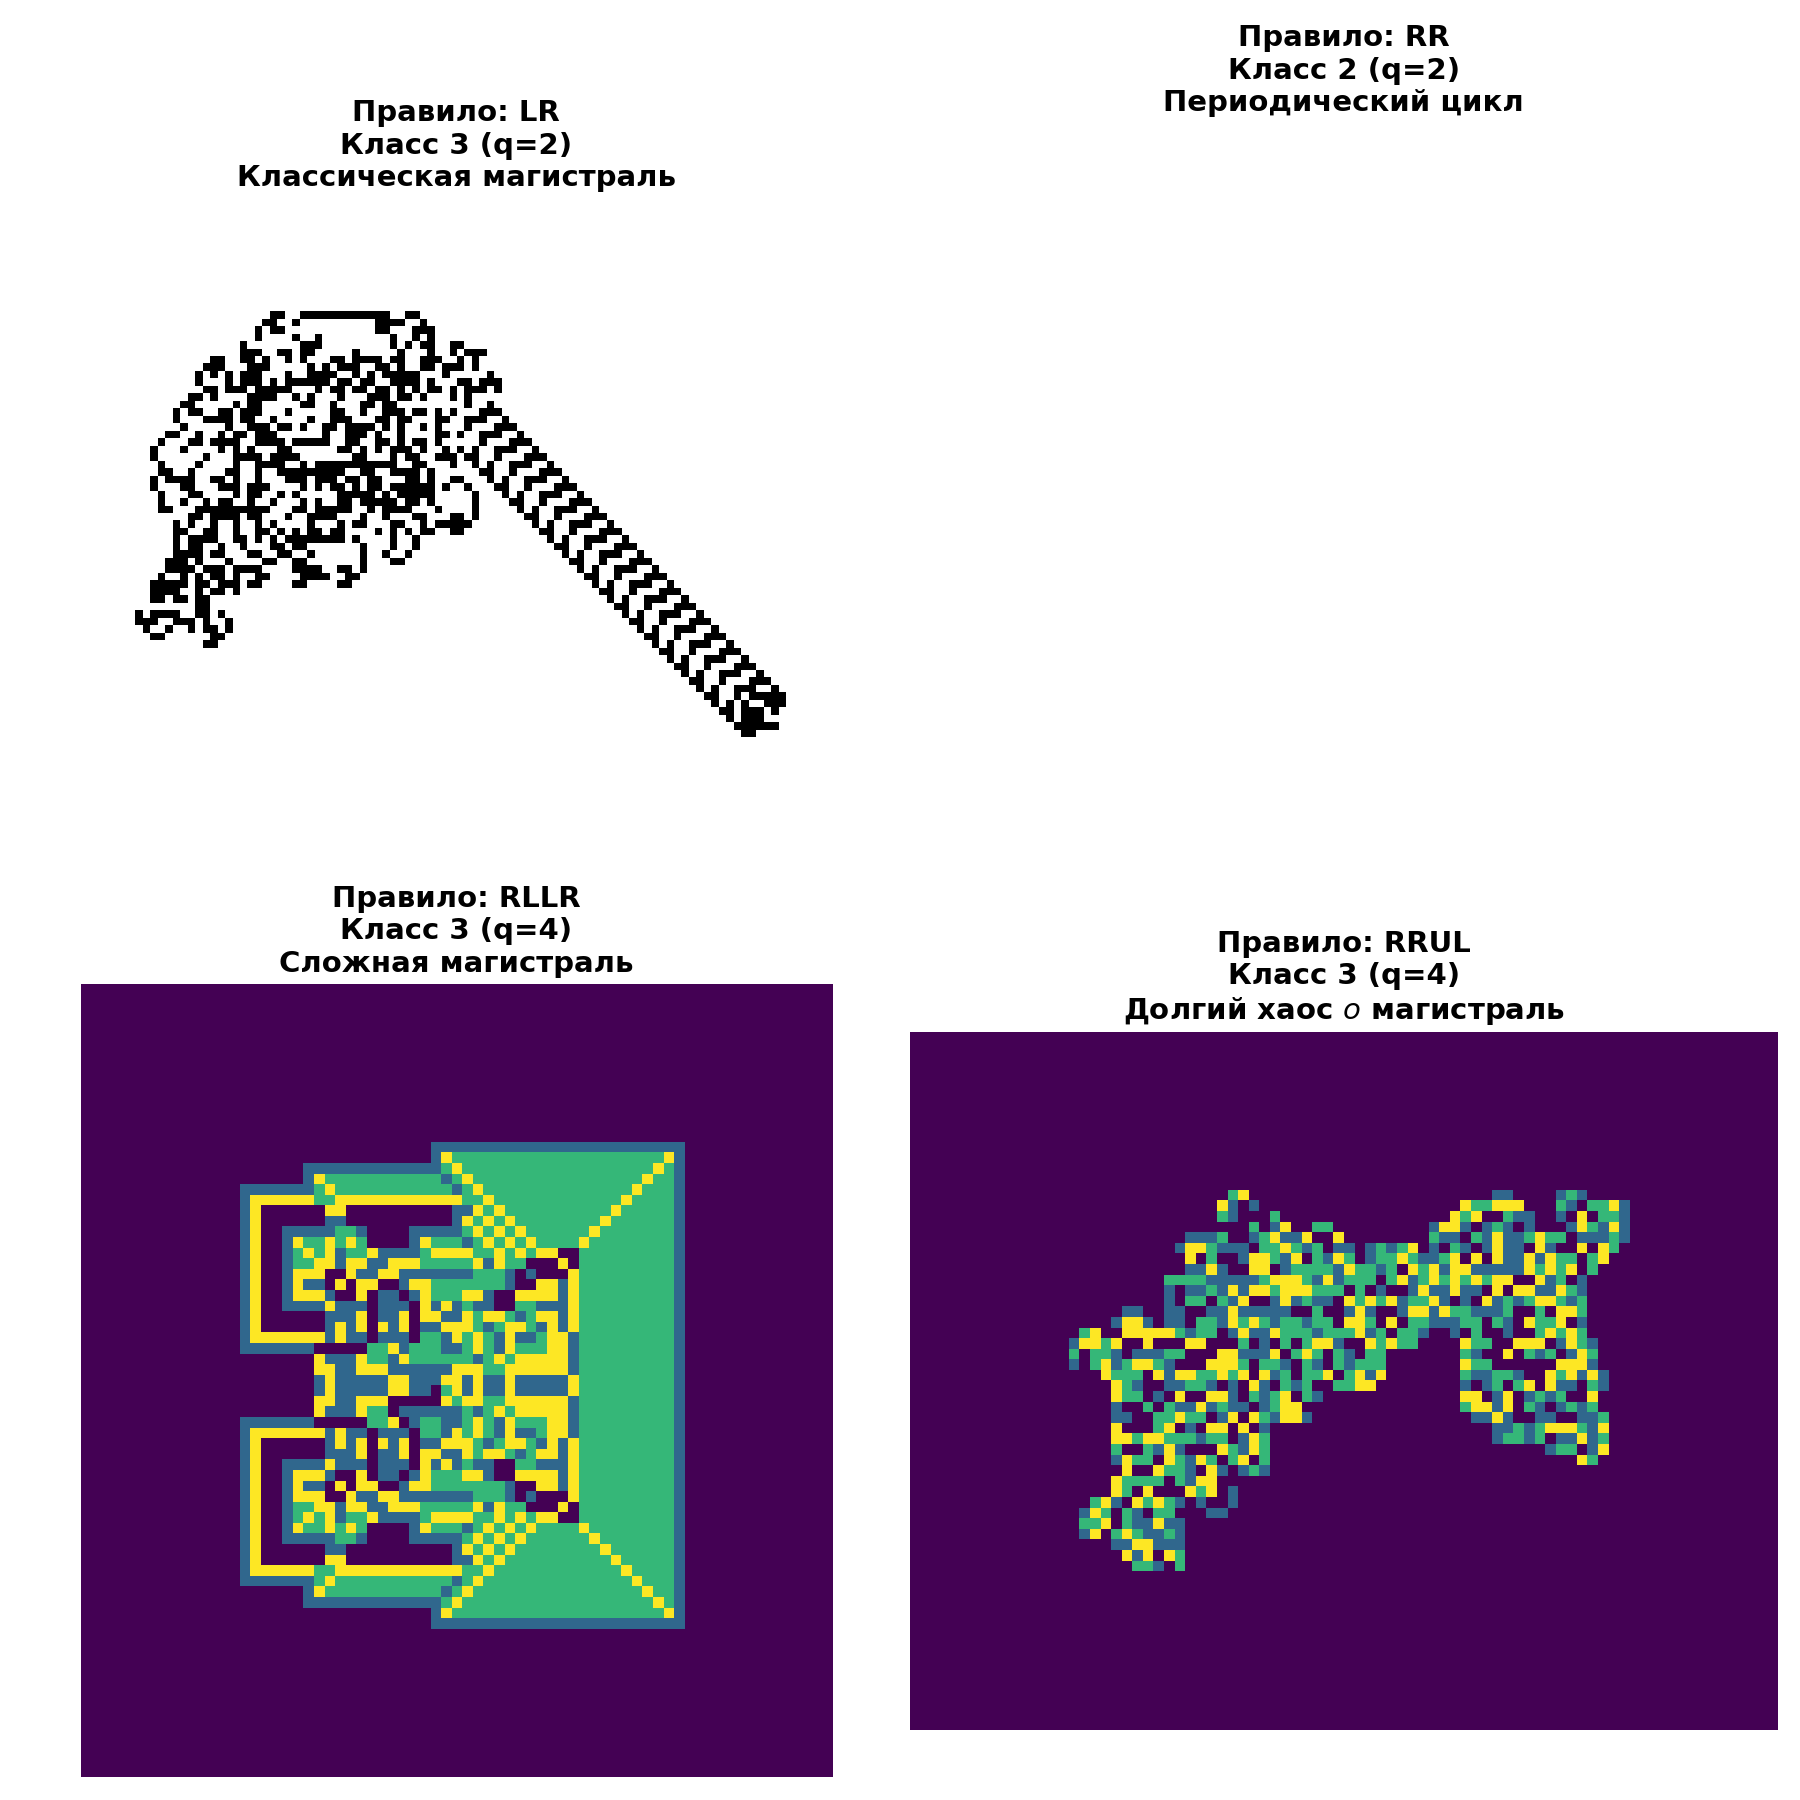
\includegraphics[width=\textwidth]{ant_gallery.png}
		\caption{Галерея режимов: классическая магистраль \texttt{LR} ($q=2$);
			пустое поле правила \texttt{RR} на шаге 200 $=25\tau$ (визуальное доказательство
			периодичности: поле вернулось в начальное состояние); структурированный фронт
			\texttt{RLLR} ($q=4$); долгий хаос правила \texttt{RRUL} ($q=4$).}
		\label{fig:gallery}
	\end{figure}
	
	\begin{figure}[H]
		\centering
		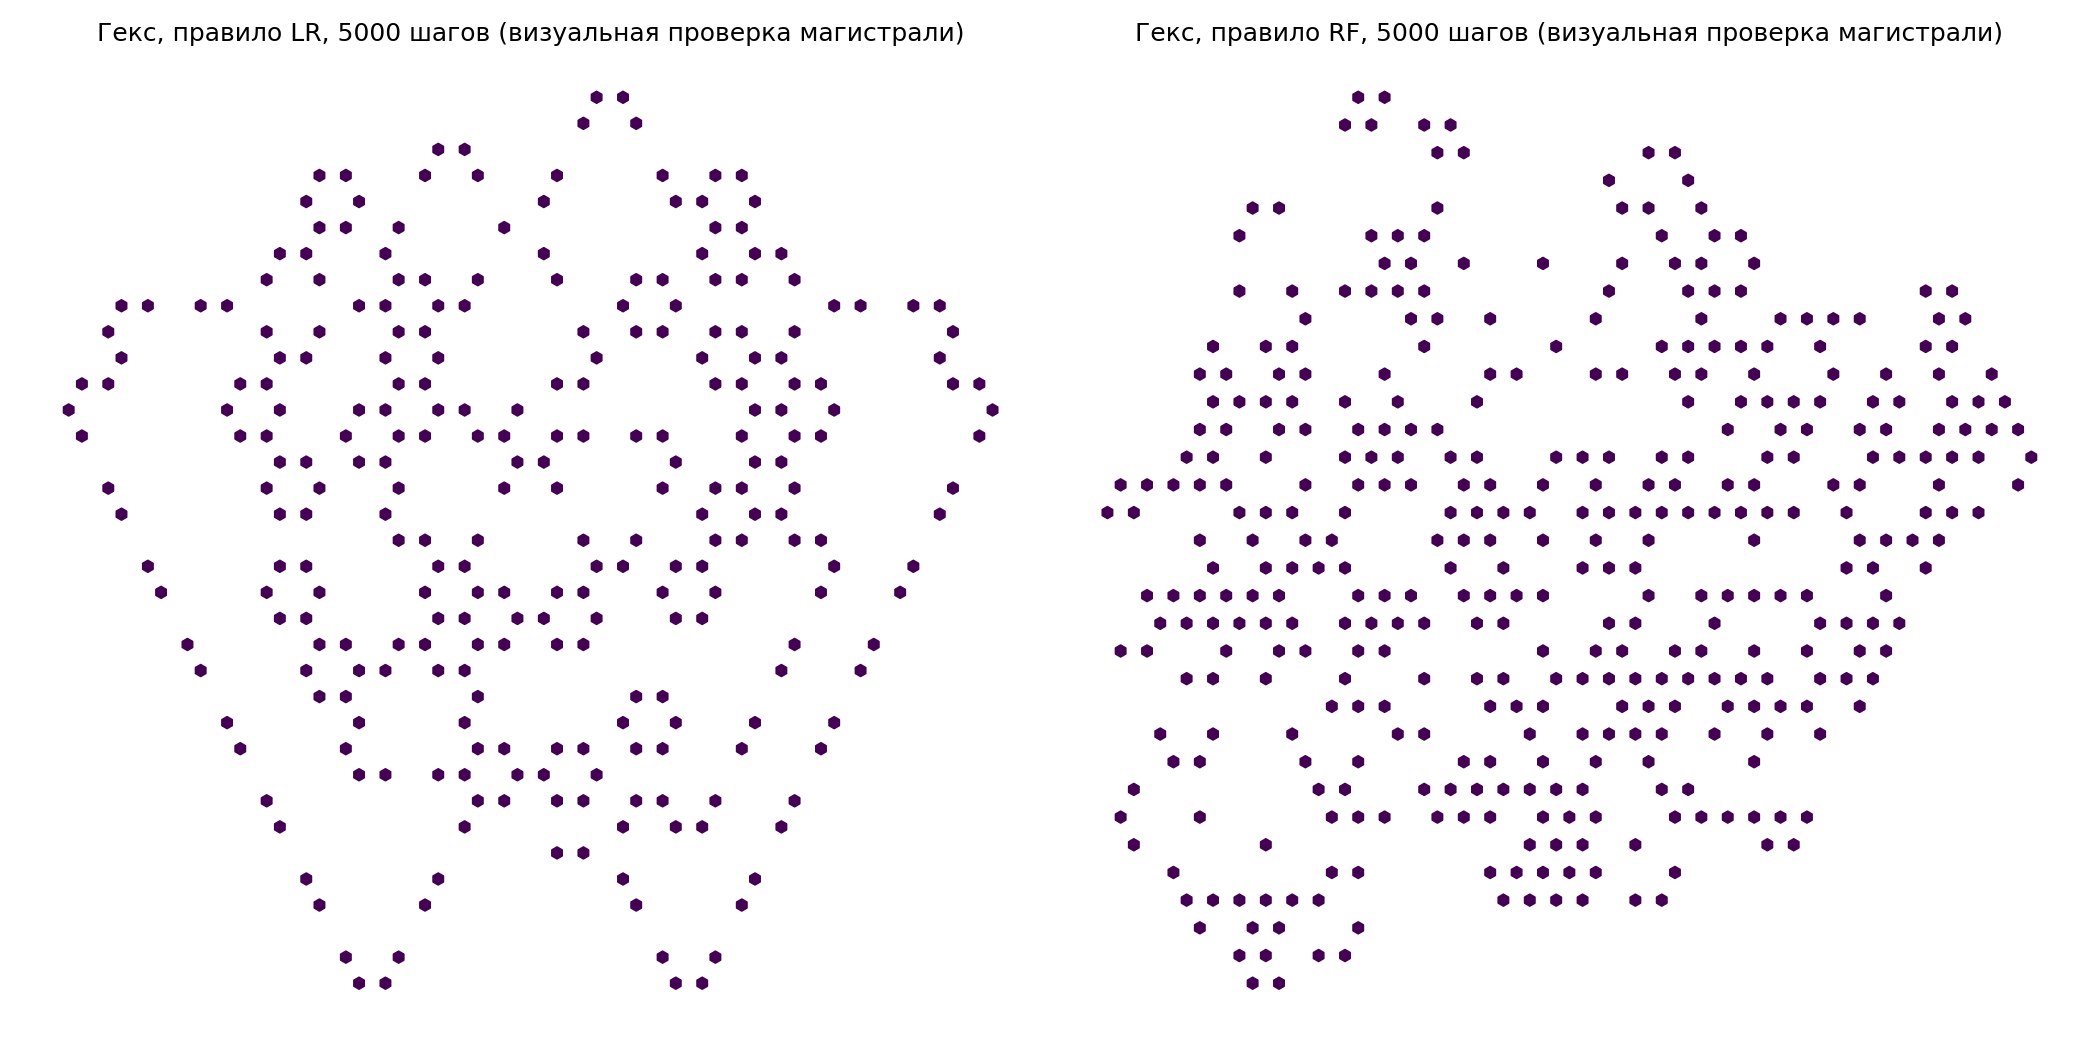
\includegraphics[width=\textwidth]{series5b_hex.png}
		\caption{Гексагональная решётка, правила \texttt{LR} и \texttt{RF}, 5000 шагов:
			широкие разреженные облака вместо дрейфующих лент --- визуальное опровержение
			<<магистралей>>, заявленных наивным детектором.}
		\label{fig:hexcloud}
	\end{figure}
	
	\begin{figure}[H]
		\centering
		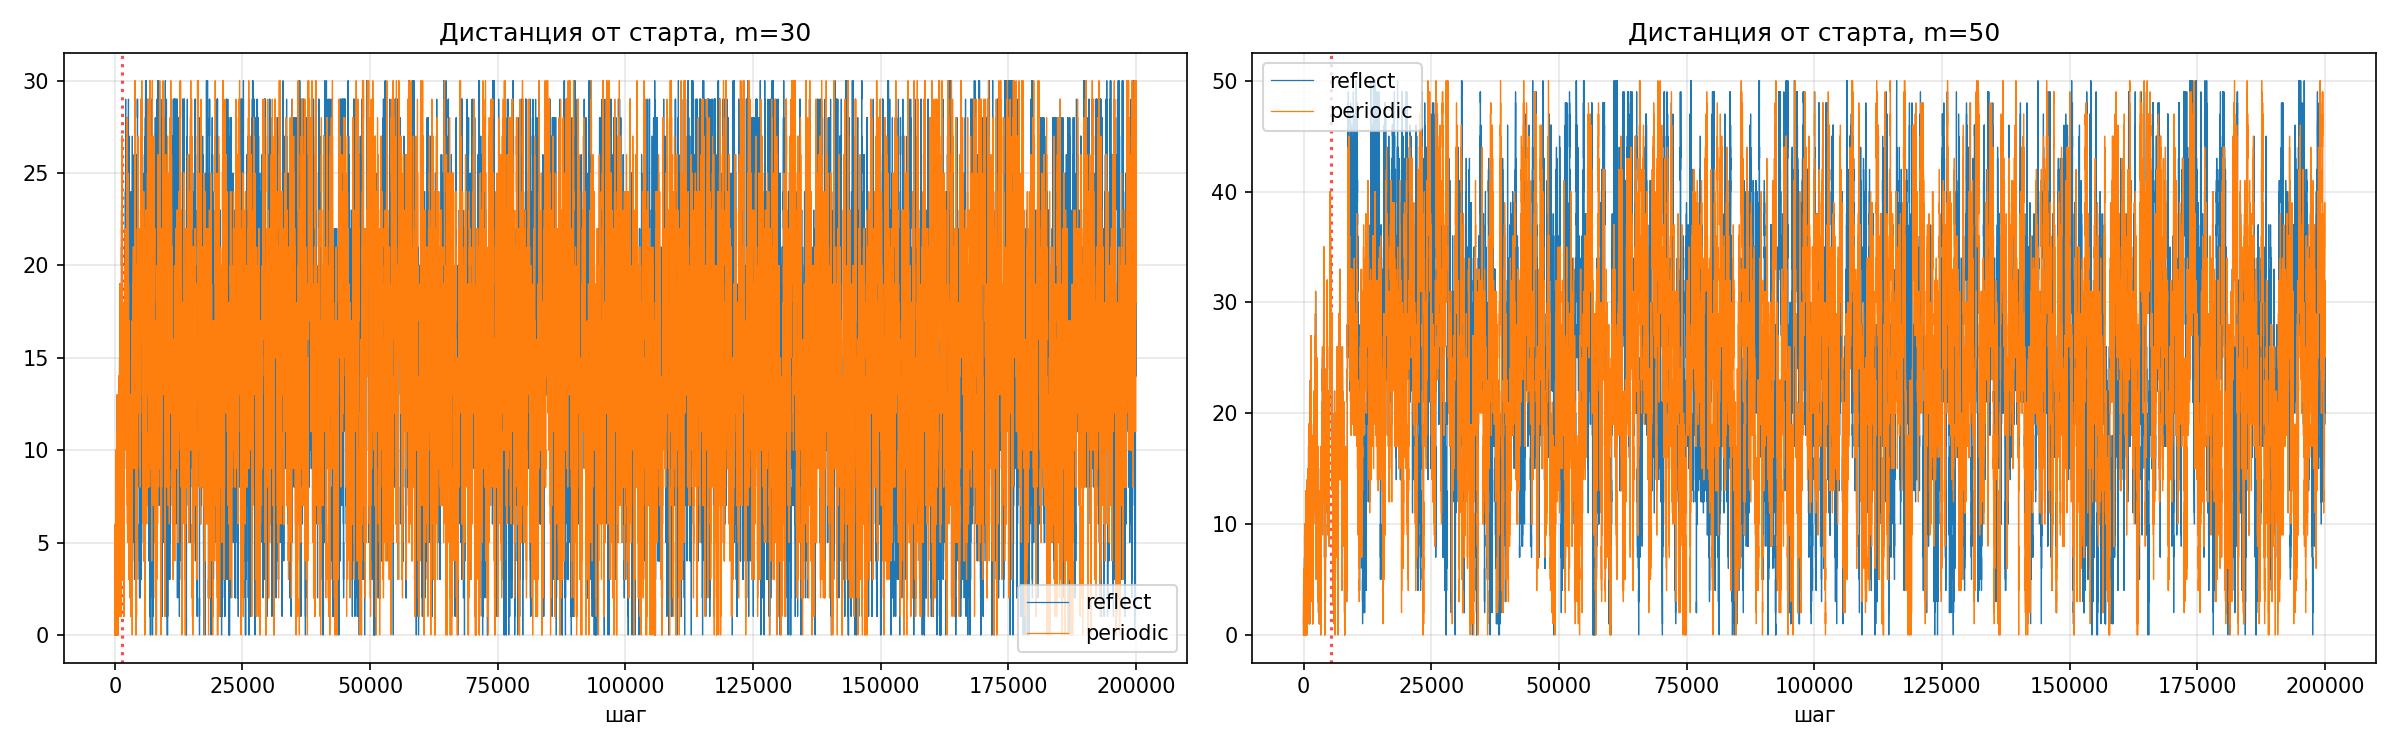
\includegraphics[width=\textwidth]{series5b_dist.png}
		\caption{Дистанция от старта в коробках $m=30$ и $m=50$: после первого контакта
			с границей (пунктир) линейный дрейф отсутствует, траектория заполняет весь
			объём; кривые отражающей и периодической границ совпадают до первого
			граничного события и расходятся после него.}
		\label{fig:dist}
	\end{figure}
	
	\begin{figure}[H]
		\centering
		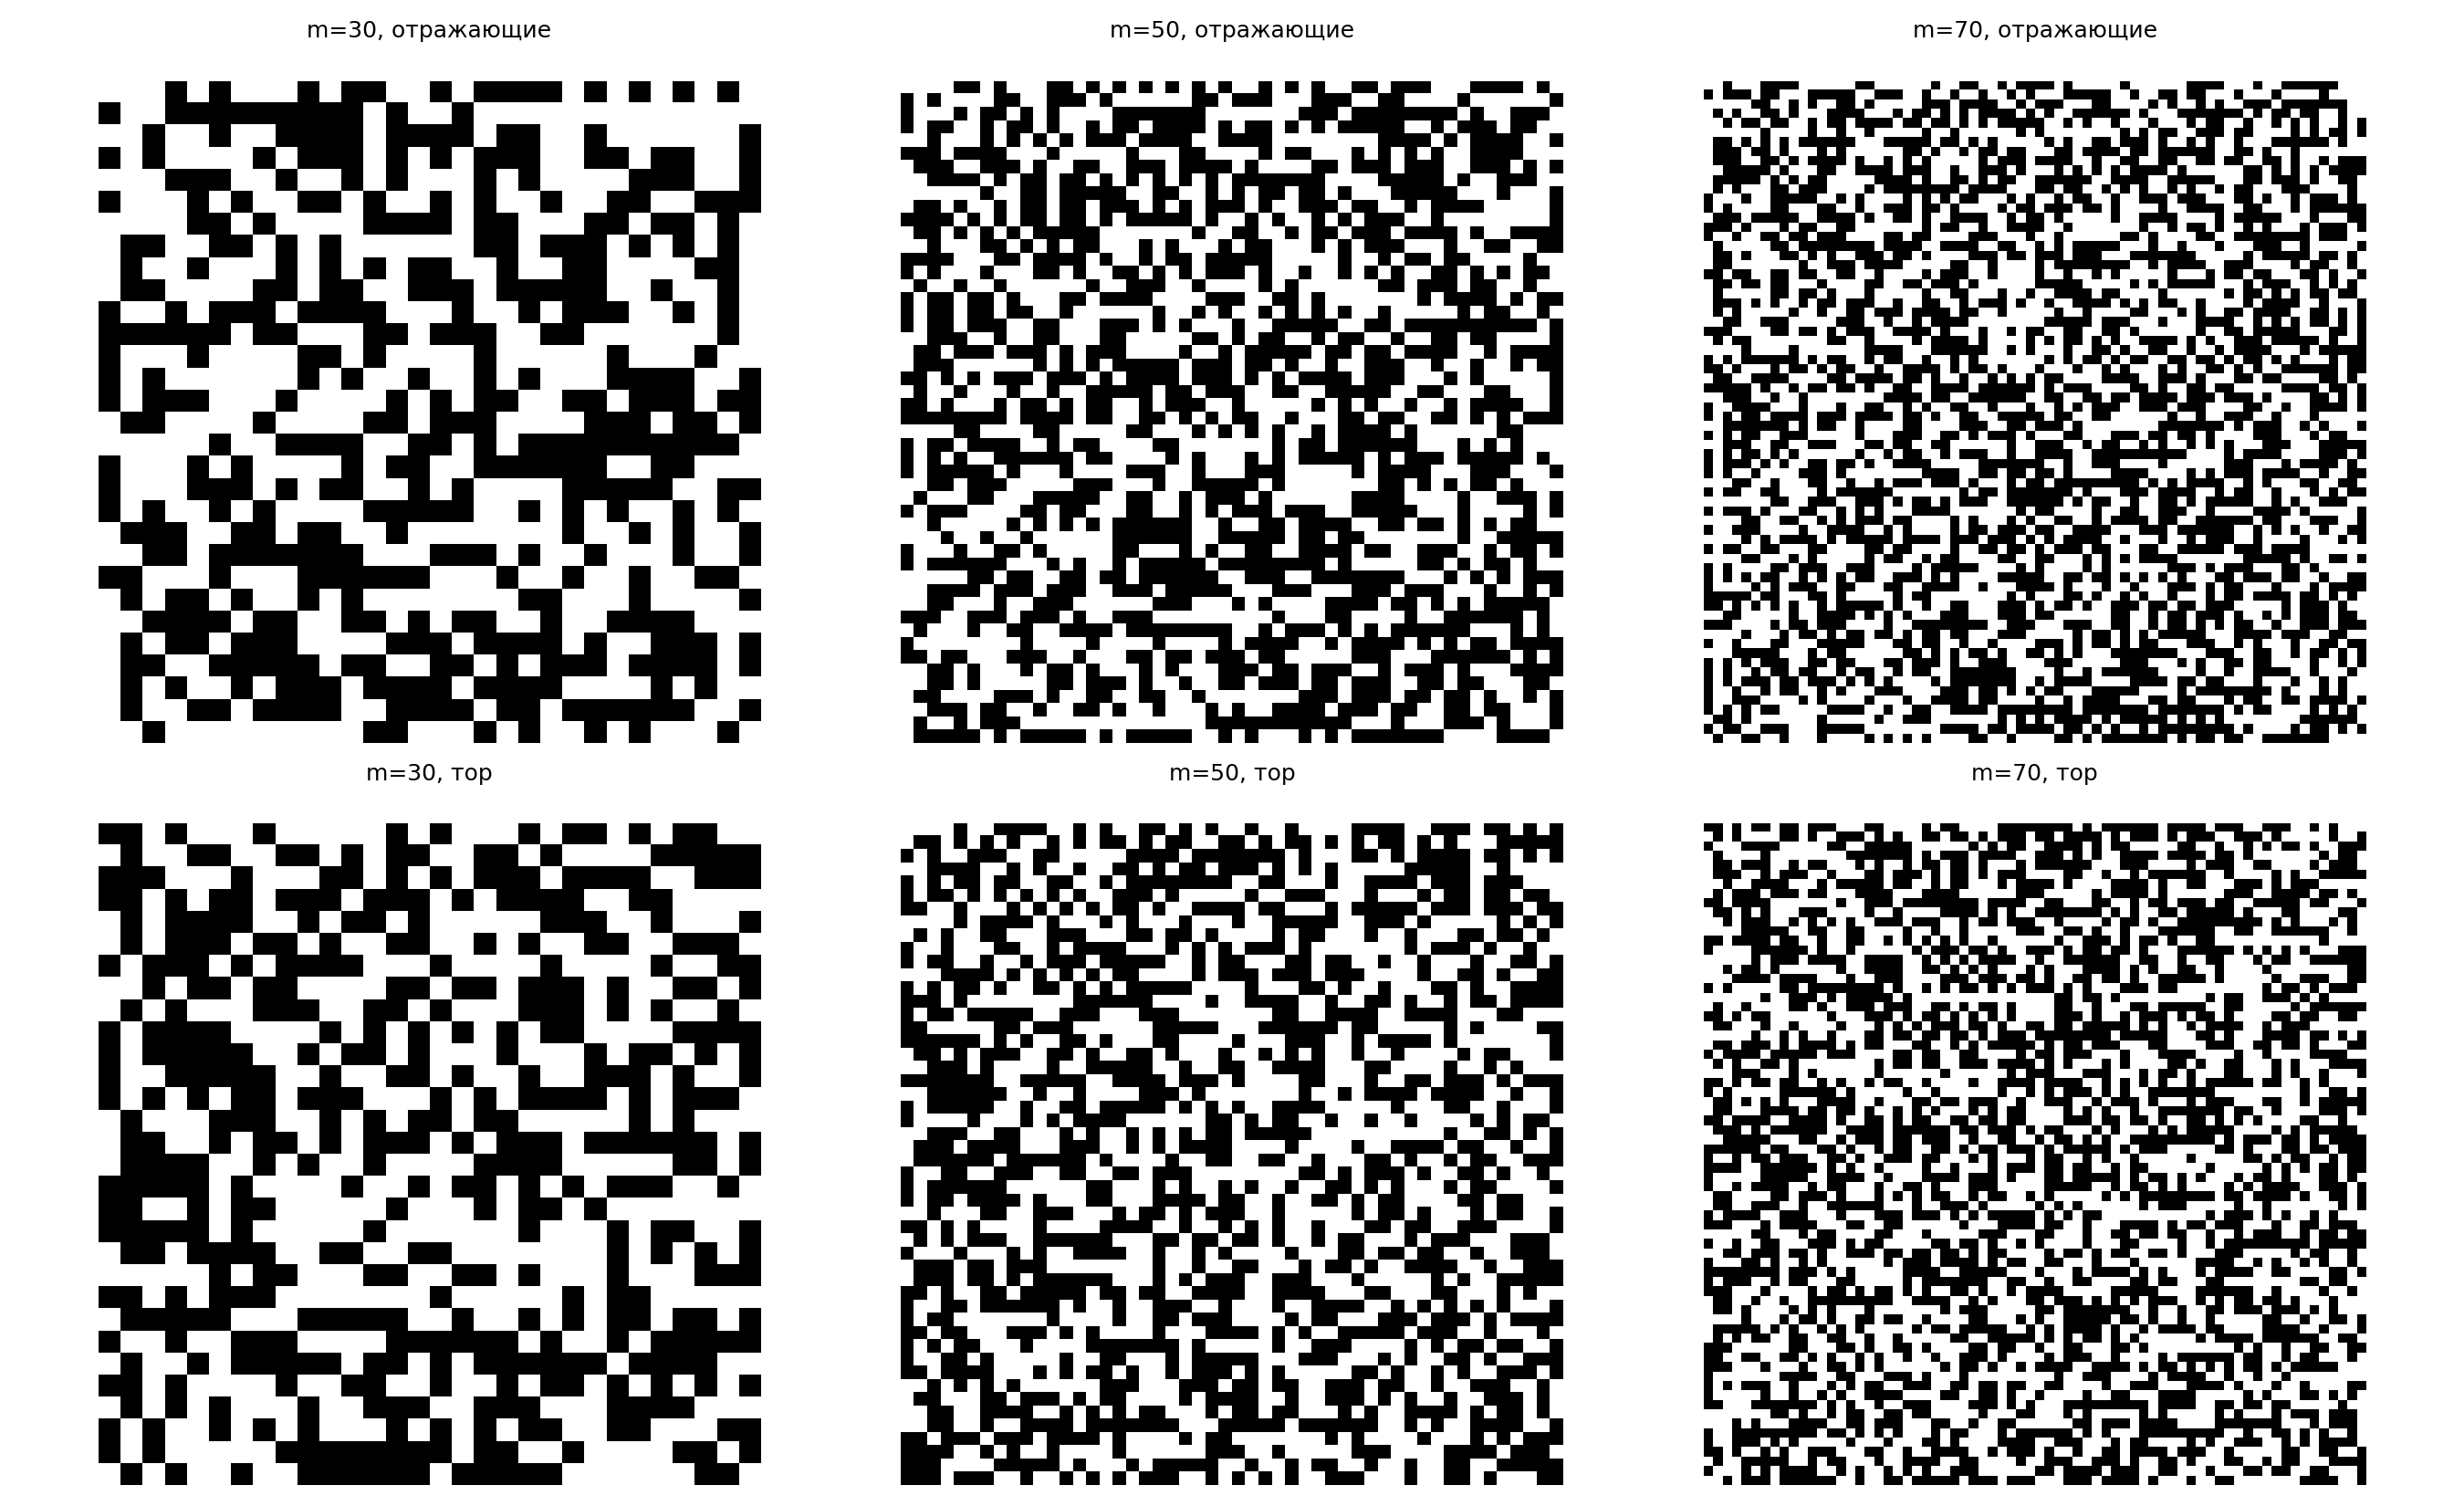
\includegraphics[width=\textwidth]{series5b_fields.png}
		\caption{Итоговые поля в коробках: верхний ряд --- отражающие границы,
			нижний --- тор; слева направо $m=30,50,70$. Граничный хаос заполняет объём;
			структура узора зависит от типа границы и размера коробки.}
		\label{fig:fields}
	\end{figure}
	
	\section{Результаты}
	
	\paragraph{Верификация измерительного инструмента как часть исследования.}
	Центральным методологическим сюжетом работы стало обнаружение систематического артефакта детектора периодичности на локальных окнах: малое окно способно демонстрировать долгую локальную квазипериодичность внутри глобально непериодической траектории. Артефакт был выявлен не внешней проверкой, а внутренней противоречивостью данных (одинаковые <<периоды>> в конфигурациях, которые заведомо не могут совпадать) и опровергнут независимым методом (сканер последовательности направлений, хэш полного состояния, визуальный контроль). Все итоговые таблицы пересчитаны эталонным методом; расхождения наивной и эталонной классификаций приведены в табл.~\ref{tab:series3},
	\ref{tab:series5a} явно.
	
	\paragraph{Предсказуемость.}
	Момент возникновения магистрали ($\approx10^4$ шагов) не выводится аналитически и получен только полным моделированием; однако после обнаружения периода будущее системы предсказуемо за $O(1)$ на запрос позиции, что иллюстрирует тезис о снижении сложности предсказания с $m\times m\times T$ до $m\times m\times\log T$ при наличии периодичности.
	
	\paragraph{Ограничения работы.} 
	Сканер периодичности охватывает $\tau\le6000$; класс~5 (симметричный рост) в верифицированной выборке не наблюдался; окрестность агента по построению модели ограничена текущей клеткой, поэтому варьирование окрестностей заменено варьированием топологии решётки (квадрат/гекс). Направления будущих работ: несколько взаимодействующих муравьёв, перебор правил при $q=5,6$ с распараллеливанием, расширенный сканер периодов.
	
	\section{Выводы}
	
	\begin{enumerate}
		\item Классический муравей Лэнгтона на квадратной решётке после хаотической фазы ($0\dots{\approx}10^4$ шагов, флуктуации расстояния 0--48, возвраты к старту) формирует магистраль с периодом $\tau=104$, вектором сноса $d=(2,2)$ и скоростью $0.03846$ кл/шаг; момент перехода измерен двумя операциональными определениями: 9977 (траектория) и 10112 (локальное поле). Гипотеза 1 подтверждена.
		\item Динамика локальна и чувствительна к фазе: возмущение вне траектории не влияет ни на одну величину; возмущение на траектории сдвигает момент перехода на $\pm1$ шаг и зеркалит магистраль; структурный шум (5\% клеток) порождает магистраль новой архитектуры ($\tau=108$, $t_{\mathrm{onset}}=13295$).
		\item С ростом $q$ спектр режимов обогащается: при $q=3$ возникает хаос (12/64 верифицированно), при $q=4$ наивный перебор выявляет также слой ограниченных режимов; доля магистралей устойчиво держится около половины пространства правил. Гипотеза 2 подтверждена.
		\item Пространство правил изрезано: точечная мутация меняет класс поведения в 58\% (база \texttt{RLLR}) и 50\% (база \texttt{LRLR}) случаев. Гипотеза 3 подтверждена.
		\item Гексагональная топология подавляет механизм построения магистрали: классическое правило магистрали не формирует (опровергнута наивная детекция $\tau=88$), доля магистралей падает с $7/16$ до $5/16$ ($q=2$) и с $30/64$ до $18/64$ ($q=3$). Гипотеза 4 подтверждена.
		\item Ограничивающие границы разрушают магистраль при первом контакте ($t_{\mathrm{wall}}\propto m^2$) и переводят систему в устойчивый граничный хаос; точные циклы за $2\cdot10^5$ шагов не обнаружены, что согласуется с гарантированной, но практически недостижимой eventual-периодичностью конечного фазового пространства. Гипотеза 5 подтверждена в уточнённой формулировке.
		\item Методологический итог: детекторы периодичности на локальных окнах ненадёжны для клеточных автоматов с агентом; корректная классификация требует траекторных или полносостоятельных критериев и перекрёстной верификации независимыми реализациями.
	\end{enumerate}
	

	
	\newpage
	\appendix
	\section{Приложение А. Ключевой фрагмент эталонного верификатора}
	
	\begin{lstlisting}
		for tau in range(1, min(tau_max, T // 3) + 1):
		k = min(T - tau, max(3 * tau, 3000))
		if np.array_equal(dirs[T-k:T-tau], dirs[T-k+tau:T]):
		j = T - k - 1
		while j >= 0 and dirs[j] == dirs[j + tau]:
		j -= 1
		s0 = j + 2                      
		d  = pos[s0 - 1 + tau] - pos[s0 - 1]
		return cls = 2 if d == (0,0) else 3, tau, s0, d
		
		key = md5(repr((r, c, d, sorted(field.items()))).encode()).digest()
		if key in seen:  return cls = 2, tau = t - seen[key]
	\end{lstlisting}
	
	\section{Приложение Б. Артефакты эксперимента}
	Все вычислительные артефакты сохранены в каталоге работы:
	\texttt{series1\_metrics.csv} (пометрический журнал Серии~1),
	\texttt{enum\_q2.json}, \texttt{enum\_q3.json}, \texttt{enum\_q4.json}
	(каталоги правил наивного перебора), \texttt{series24.json} (Серии~2 и~4),
	\texttt{ant\_gallery.png}, \texttt{series5b\_fields.png},
	\texttt{series5b\_dist.png}, \texttt{series5b\_hex.png} (иллюстрации).
	
\end{document}